\documentclass[10pt, aspectratio=169]{beamer}

% Modern theme
\usetheme[progressbar=frametitle]{metropolis}
\usepackage{appendixnumberbeamer}
\usepackage{booktabs}
\usepackage[scale=2]{ccicons}
\usepackage{graphicx}
\usepackage{xcolor}
\usepackage{amsmath}
\usepackage{algorithm2e}

\title{Black-box Active Learning for Discovering New Explanations}
\subtitle{Application to Complex System Exploration}
\date{Derivative-Free Optimization Symposium}
\author{Paul Saves \inst{1} \and Nicolas Verstaevel \inst{1} \and Benoit Gaudou \inst{1}}
\institute{\inst{1} Université Toulouse Capitole, IRIT, France}

\begin{document}

\maketitle

\begin{frame}{Table of contents}
  \setbeamertemplate{section in toc}[sections numbered]
  \tableofcontents[hideallsubsections]
\end{frame}

\section{Introduction \& Context}

\begin{frame}[fragile]{The Computational Bottleneck of ABMs}
  \textbf{Exploring Agent-Based Models (Schelling, Cireco):}
  \begin{itemize}
    \item \textbf{Computational Expense:} A single simulator run takes significant time. High-dimensional mapping via LHS is intractable.
    \item \textbf{Black-Box \& Non-Differentiable:} No gradients to guide the search towards interesting behaviors.
    \item \textbf{The "Needle in a Haystack":} Traditional Active Learning minimizes \textit{prediction uncertainty}, wasting simulations in noisy but homogeneous regions while missing critical tipping points.
  \end{itemize}
\end{frame}

\begin{frame}[fragile]{The Core Concept: Explanatory Diversity}
  \textbf{The Shift:} Stop hunting for \textit{prediction uncertainty}; start hunting for \textit{explanatory novelty}.
  
  \vspace{0.5cm}
  Instead of looking only at the prediction $y$, we extract feature contribution profiles using Explainable AI (SHAP):
  $$S(x) = \text{SHAP}(f, x)$$
  
  \textbf{The Goal:} Explicitly sample regions where the internal logic (the explanation) of the model fundamentally changes.
\end{frame}

\section{Pipeline \& Innovations}

\begin{frame}[fragile]{The Active Learning Pipeline Architecture}
  \textbf{Step 1: Initial DoE.} Evaluate $N_{init}$ points via LHS.\\
  \textbf{Step 2: Primary Surrogate.} Train Kriging GP on $\{x_{doe}, y_{doe}\}$.\\
  \textbf{Step 3: Proxy SHAP.} Sample thousands of cheap points, compute ExactSHAP via the primary surrogate as a proxy.\\
  \textbf{Step 4: Novelty Calculation.} Calculate SHAP Novelty metric.\\
  \textbf{Step 5: Multi-Fidelity Surrogate.} Train Multi-Fidelity Kriging (MFK) on the Novelty metric.\\
  \textbf{Step 6: Acquisition.} Hybrid Acquisition Function selects the next optimal point $\rightarrow$ Evaluate on True ABM.
\end{frame}

\begin{frame}[fragile]{Algorithmic Innovations (I): Fast Cosine Proxy}
  \textbf{From Slow KDE to Fast Cosine Proxy:}
  \begin{itemize}
      \item The initial theory relied on high-dimensional Kernel Density Estimation (KDE) on SHAP values:
      $$p_{SHAP}(S(x)) = \frac{1}{N} \sum_{i=1}^N K_h(S(x) - S(x_i))$$
      \item \textbf{The Upgrade:} KDE suffers from the curse of dimensionality and is computationally prohibitive.
      \item \textbf{The Solution:} We implemented a \textbf{Fast Density Proxy via Cosine Distance} (Nearest Neighbors) in SHAP space. High cosine distance translates directly to high explanatory novelty.
  \end{itemize}
\end{frame}

\begin{frame}[fragile]{Algorithmic Innovations (II): Dynamic Hybrid Acquisition}
  \textbf{Balancing the Exploration (Dynamic-US):}
  
  Our optimizer dynamically weighs Global Exploration against Explanatory Novelty.
  $$a_{Dynamic}(x) = (1 - \lambda) \cdot \text{Norm}(\sigma^2_{GP}(x)) + \lambda \cdot \text{Norm}(\text{EI}_{MFK}(x))$$
  
  \begin{itemize}
      \item Over iterations, $\lambda$ shifts from $0.0$ (pure Space-US) to $1.0$ (pure SHAP-US).
      \item \textbf{Result:} It first maps global macroscopic behavior, then pivots strategically to isolate the complex, multi-dimensional \textbf{tipping points}.
  \end{itemize}
\end{frame}

\section{Results \& Analysis}

\begin{frame}[fragile]{Hunting Tipping Points in PCA Space}
  \begin{columns}
    \begin{column}{0.4\textwidth}
      \begin{itemize}
        \item Traditional methods (LHS, Space-US) sample densely in the homogeneous bulk.
        \item Our method (\textbf{SHAP-US} and \textbf{Dynamic-US}) efficiently populates the boundaries and critical tipping points.
      \end{itemize}
    \end{column}
    \begin{column}{0.6\textwidth}
      \begin{figure}
        \centering
        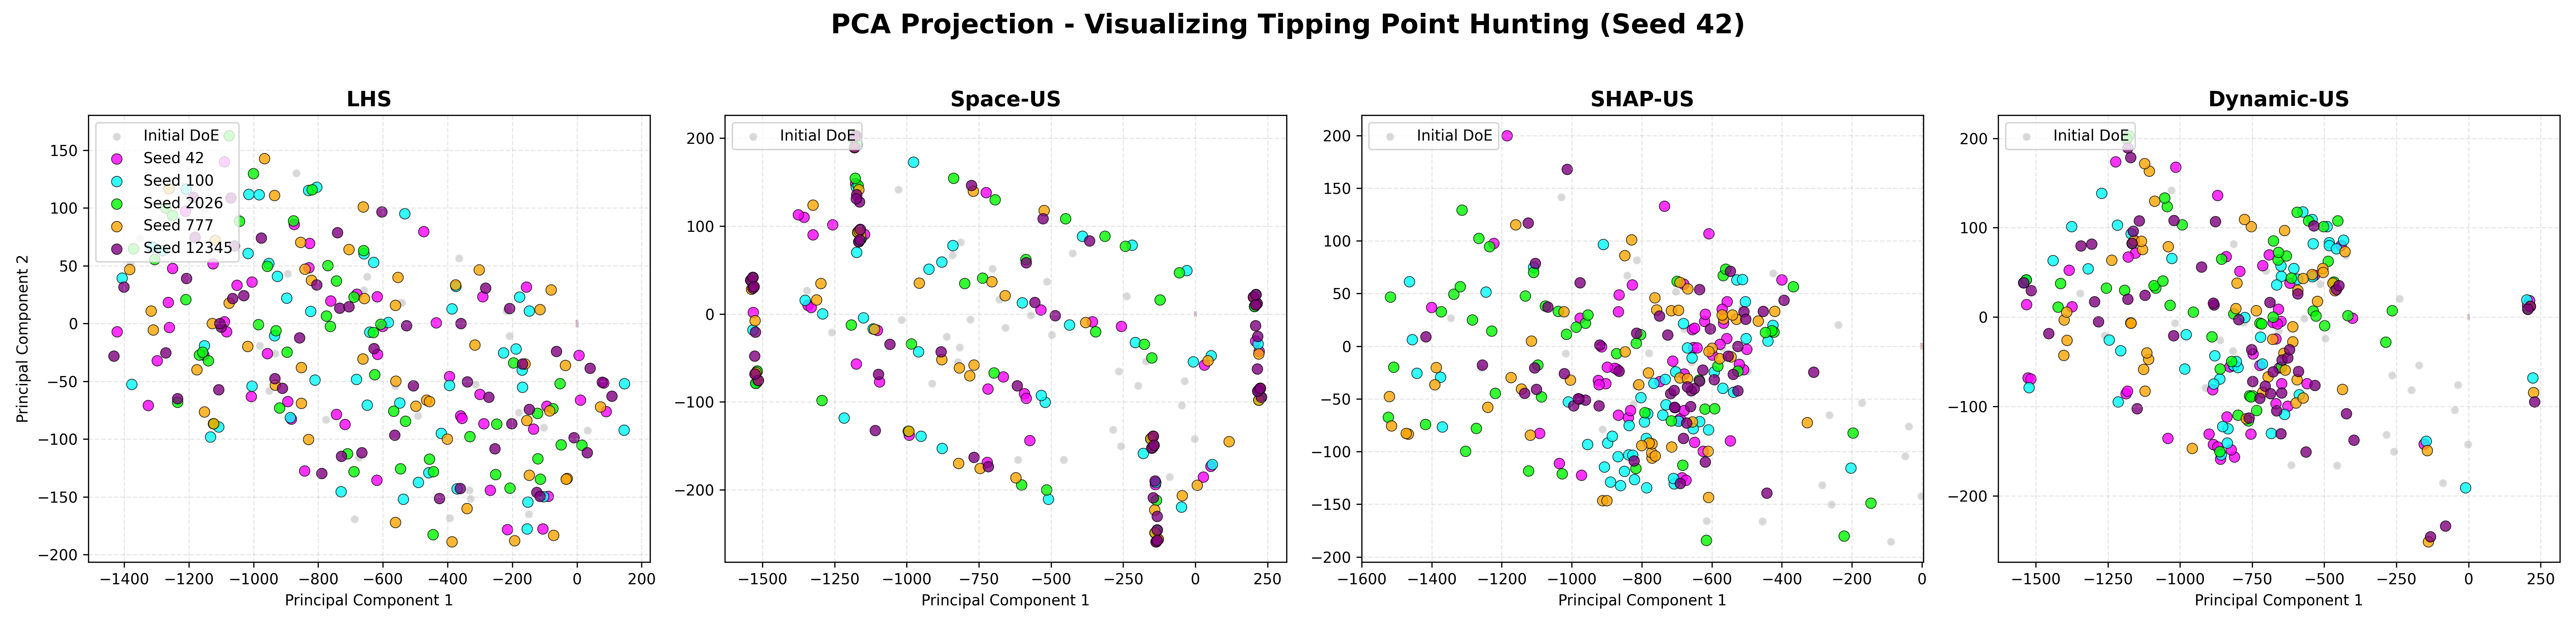
\includegraphics[width=\textwidth]{cireco_final_tipping_points_pca.png}
        \caption{Exploration of the Cireco Model (PCA space)}
      \end{figure}
    \end{column}
  \end{columns}
\end{frame}

\begin{frame}[fragile]{Convergence and Stability over Time}
  \begin{columns}
    \begin{column}{0.5\textwidth}
      \begin{figure}
        \centering
        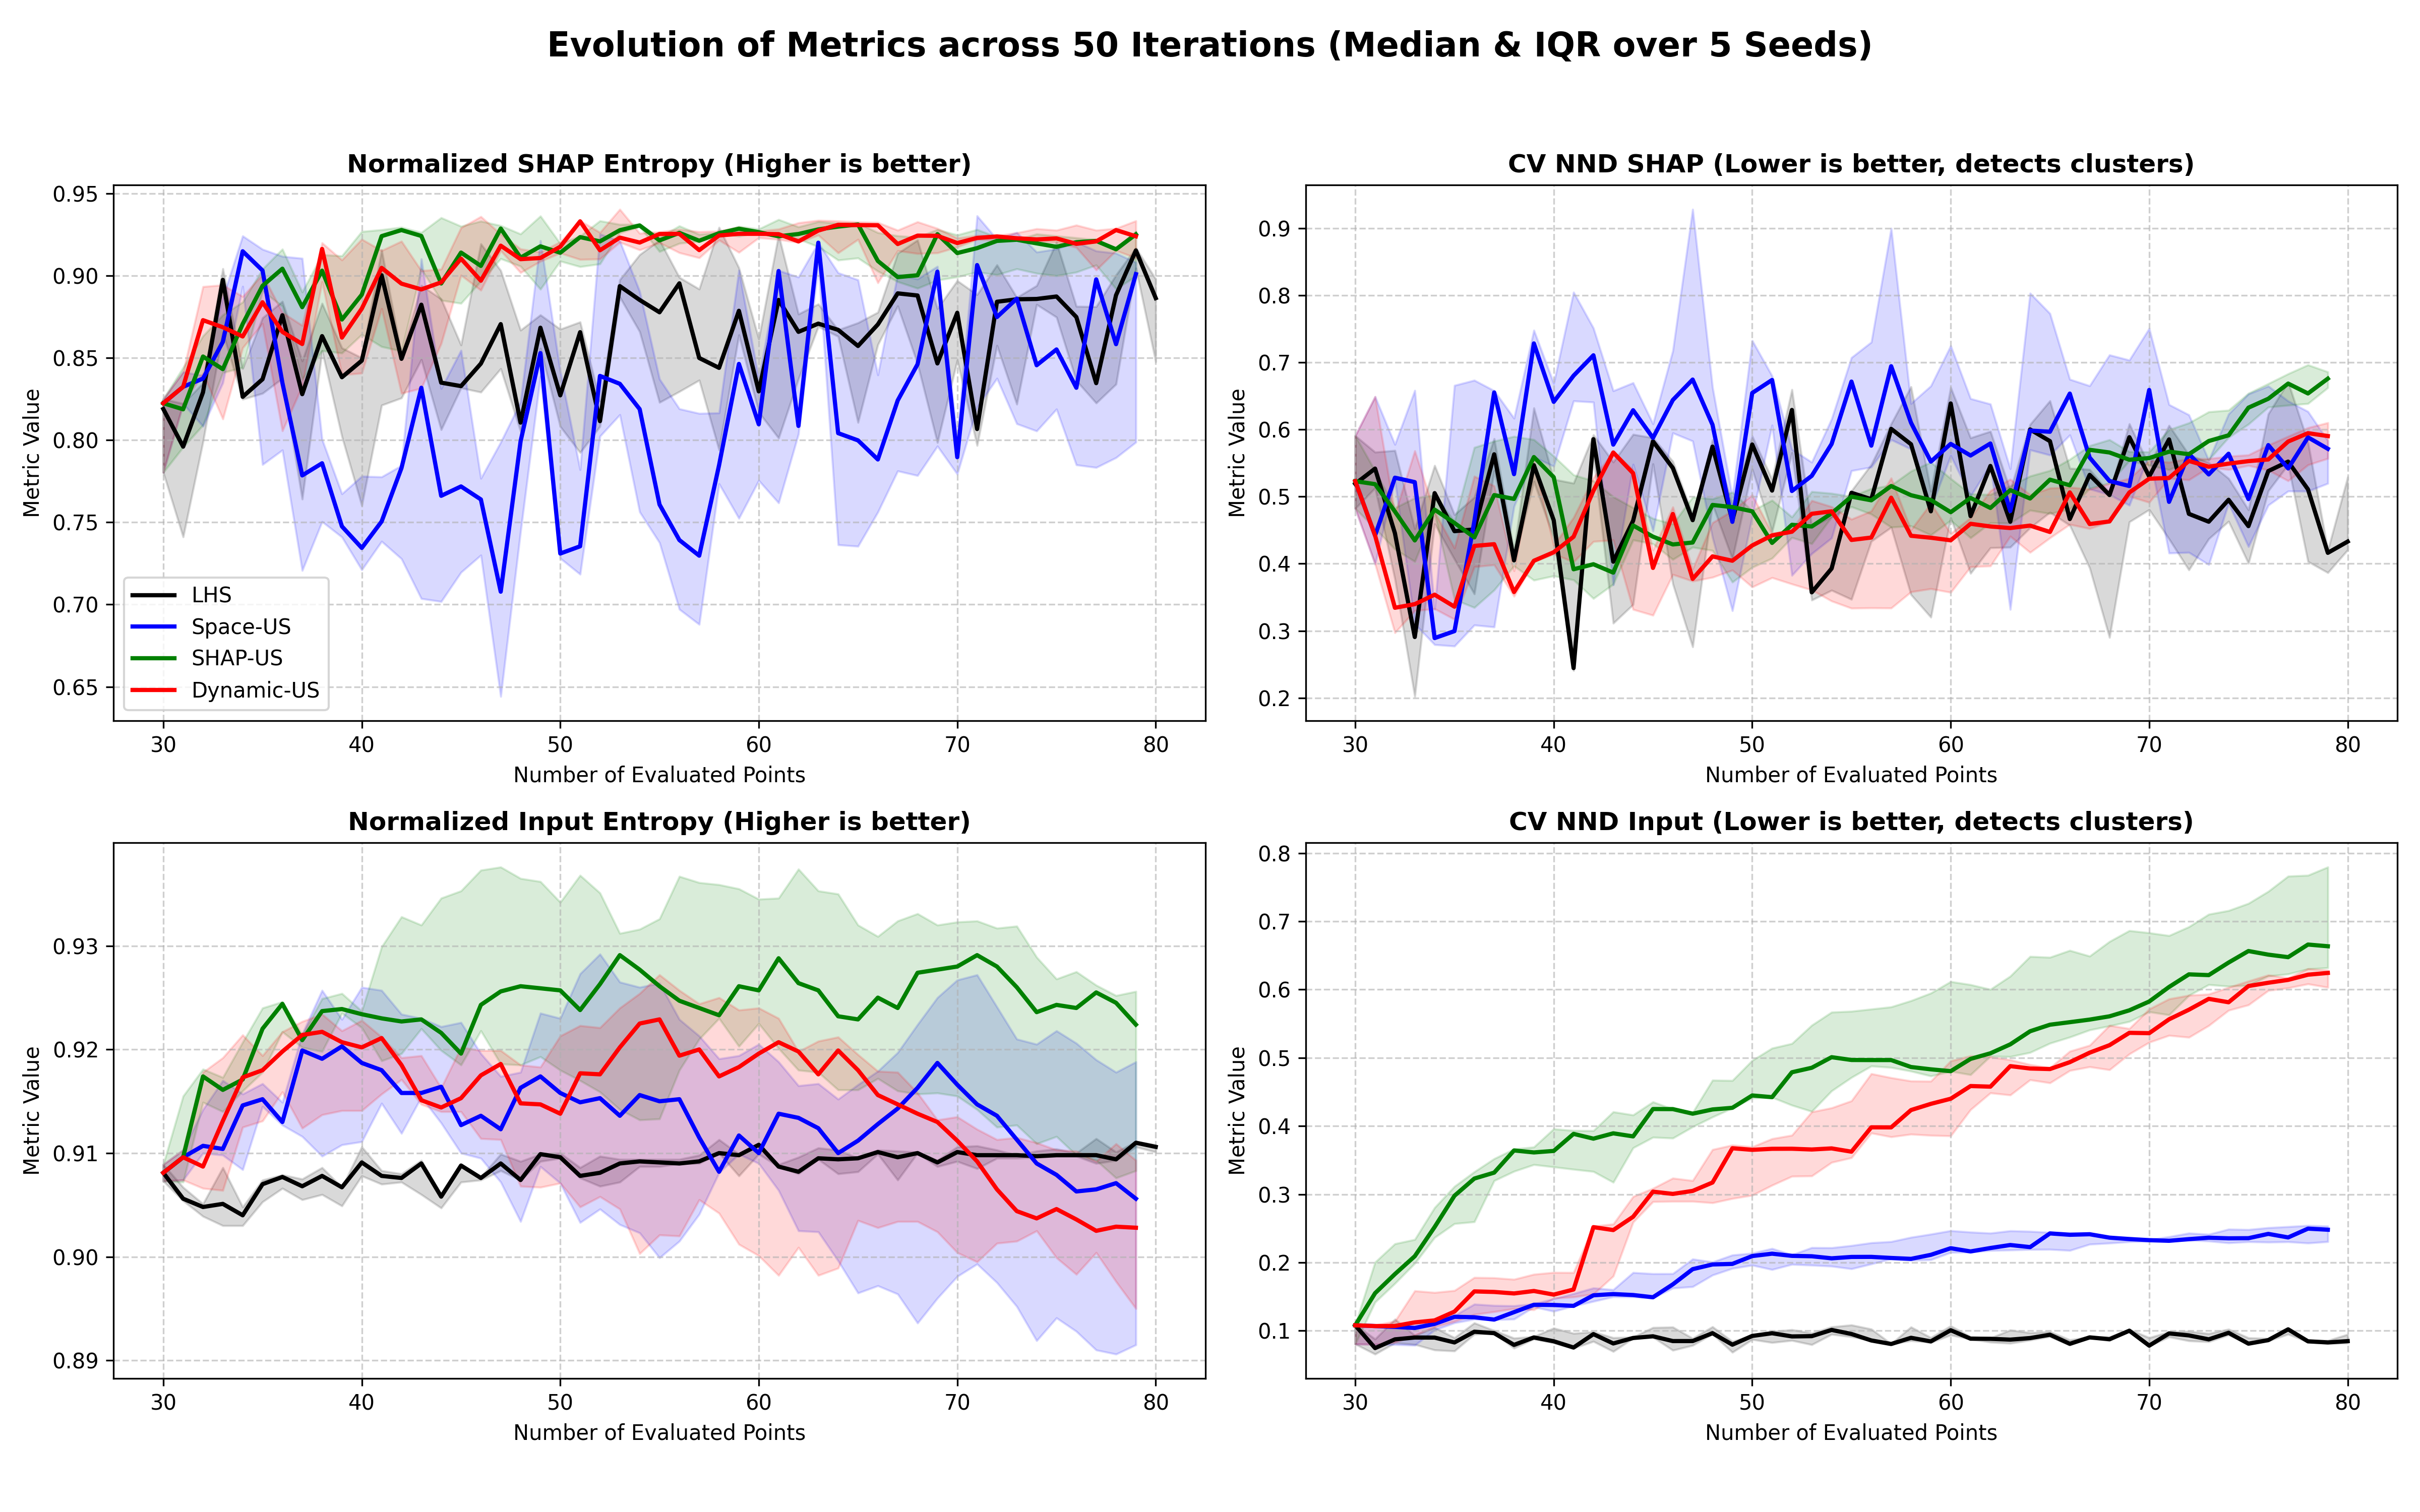
\includegraphics[width=0.9\textwidth, height=0.7\textheight, keepaspectratio]{schelling_final_all_metrics_evolution.png}
      \end{figure}
    \end{column}
    \begin{column}{0.5\textwidth}
      \begin{itemize}
        \item \textbf{Dynamic-US (Red)} matches the high explanatory diversity (SHAP entropy) of SHAP-US.
        \item Crucially, it avoids the catastrophic crash in physical input entropy seen in pure SHAP-US.
        \item It converges reliably without pathological spatial clustering.
      \end{itemize}
    \end{column}
  \end{columns}
\end{frame}

\begin{frame}[fragile]{Under the Hood: How Dynamic-US Samples Differently}
  \begin{columns}
    \begin{column}{0.5\textwidth}
      \begin{figure}
        \centering
        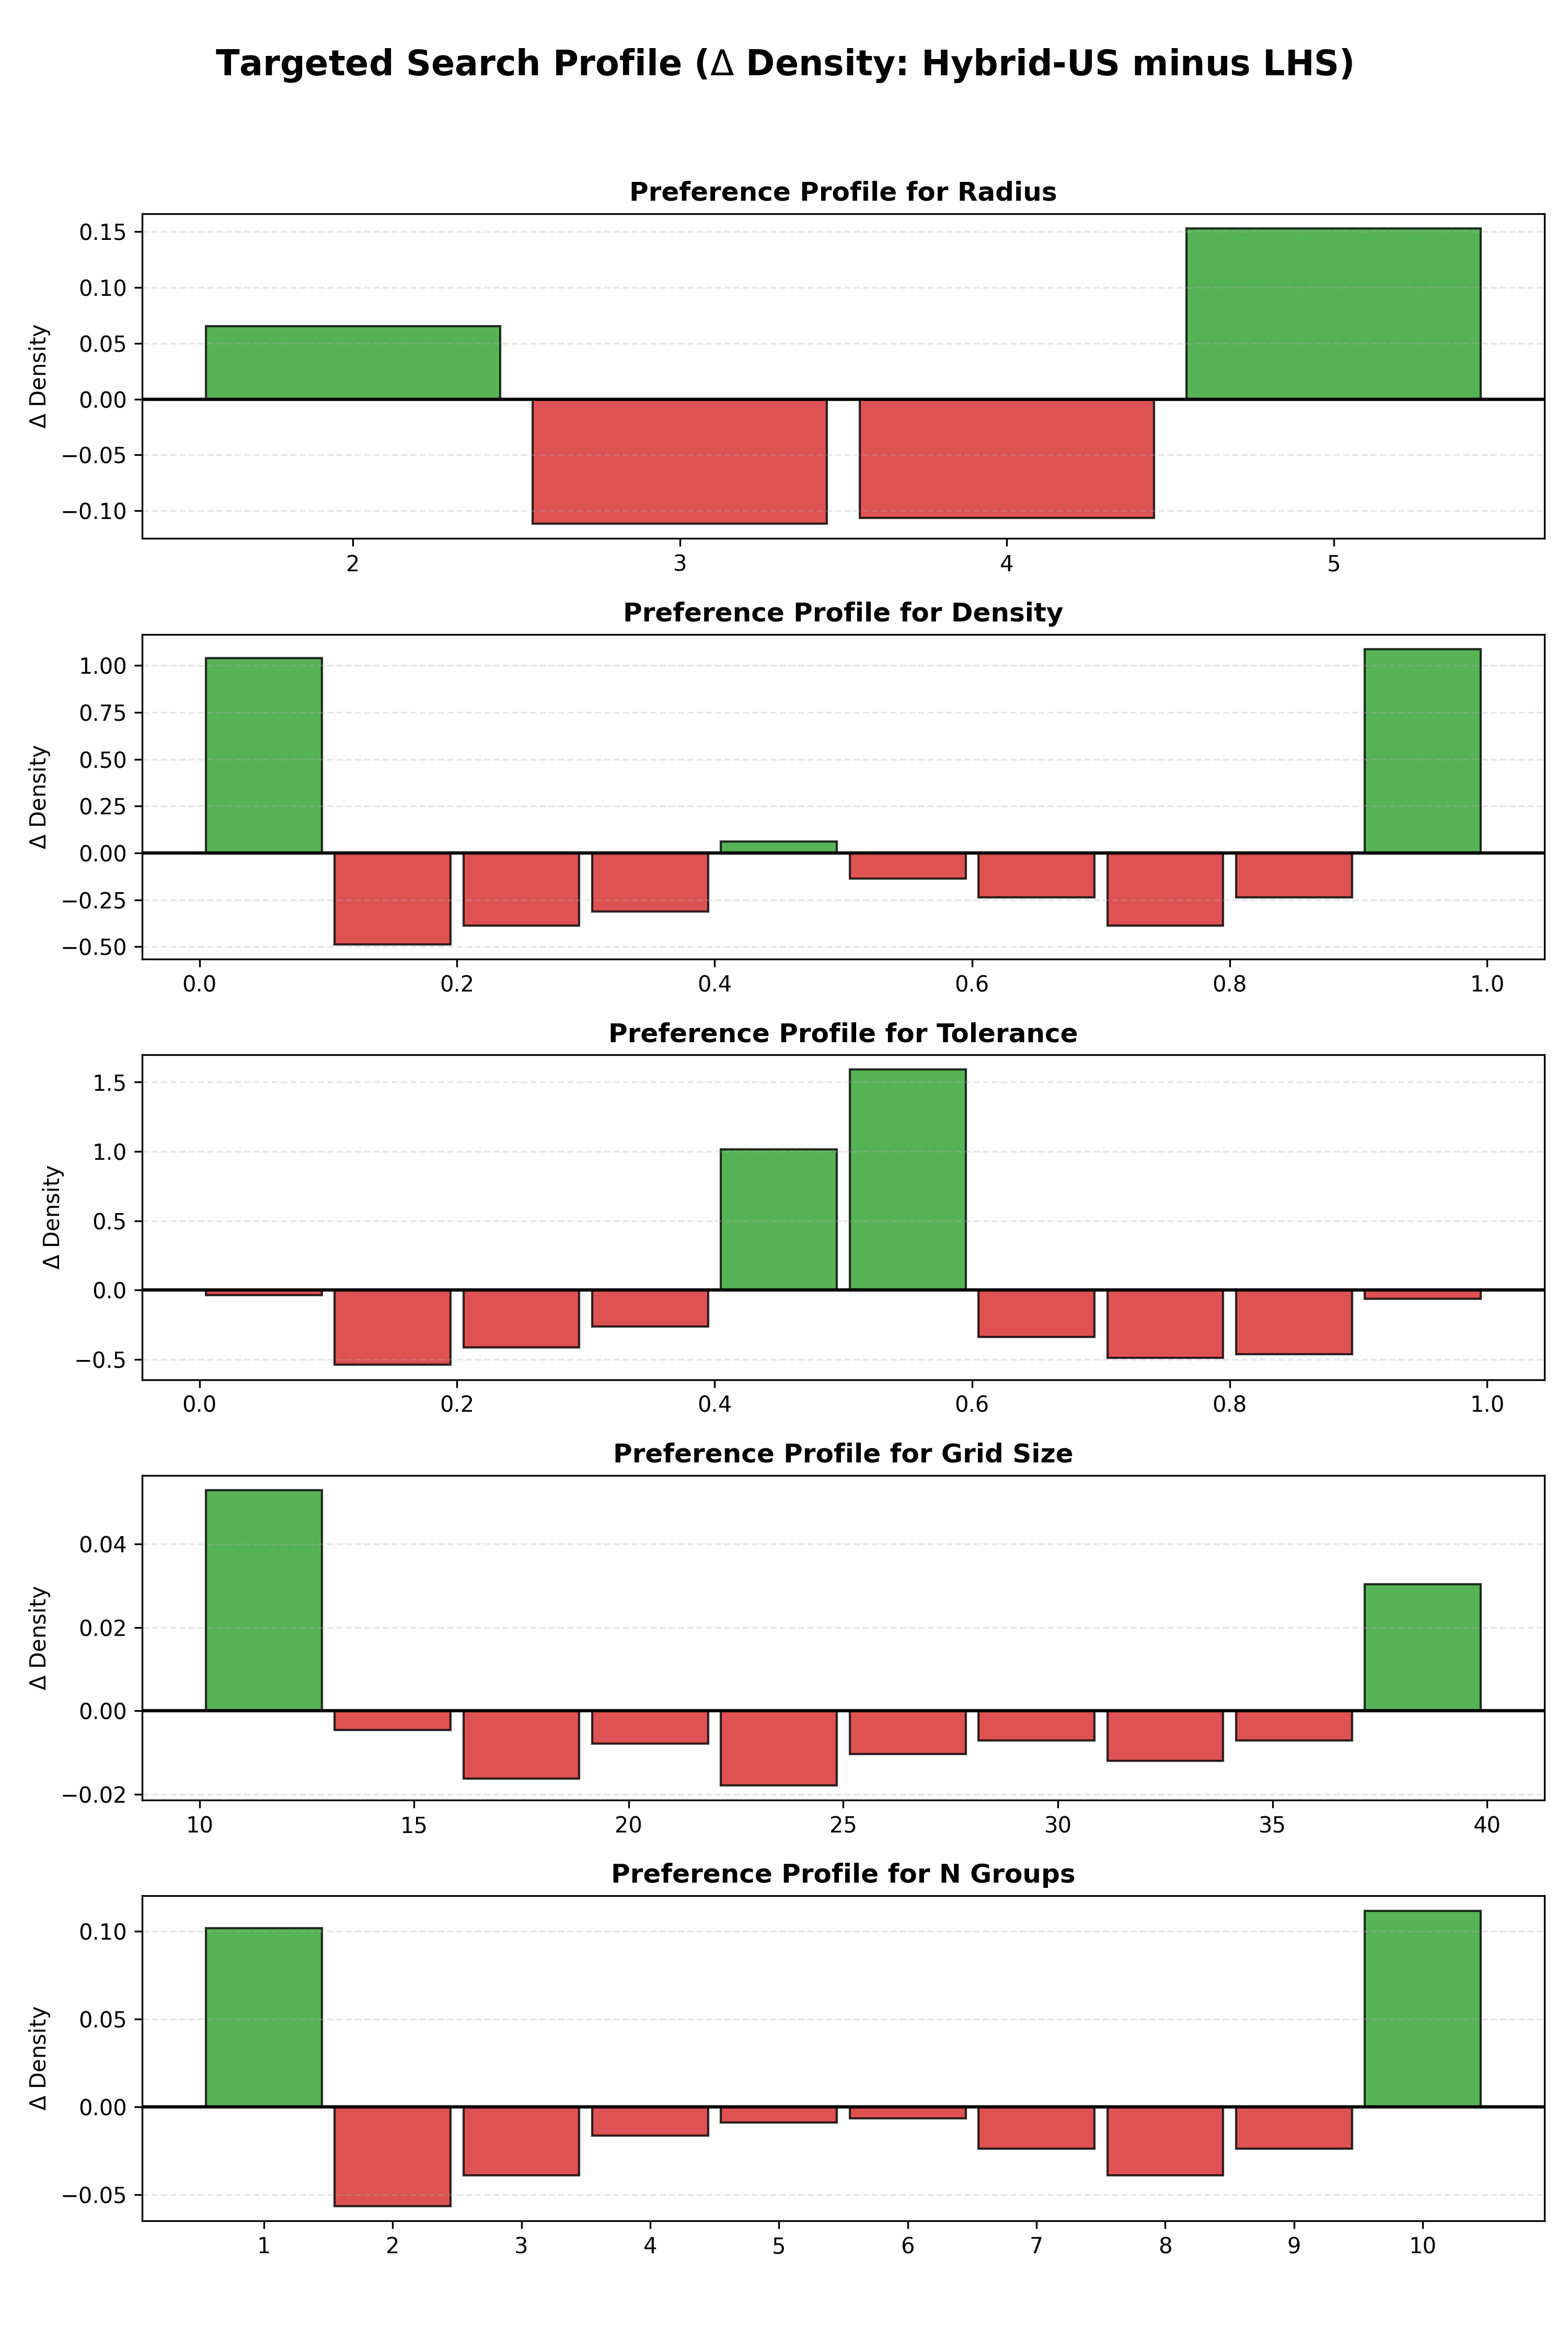
\includegraphics[width=0.9\textwidth, height=0.7\textheight, keepaspectratio]{schelling_final_hybrid_diff_profile.png}
      \end{figure}
    \end{column}
    \begin{column}{0.5\textwidth}
      \begin{itemize}
        \item Shows the Delta Density (\textbf{Dynamic-US minus LHS}).
        \item \textbf{Green:} Active learner intentionally over-sampled this region.
        \item \textbf{Red:} Actively ignored.
        \item Validates that Dynamic-US aggressively targets specific narrow bands (e.g., Tolerance around 0.5) where the tipping points live.
      \end{itemize}
    \end{column}
  \end{columns}
\end{frame}

\begin{frame}[fragile]{Dual Space Efficiency}
  \begin{columns}
    \begin{column}{0.4\textwidth}
      \begin{itemize}
        \item \textbf{Physical Diversity} vs \textbf{Explanatory Diversity}.
        \item Dynamic-US achieves a rapid gain in explanatory entropy, proving it discovers diverse causal mechanisms faster.
        \item Background dots represent 250 iterations across 5 seeds.
      \end{itemize}
    \end{column}
    \begin{column}{0.6\textwidth}
      \begin{figure}
        \centering
        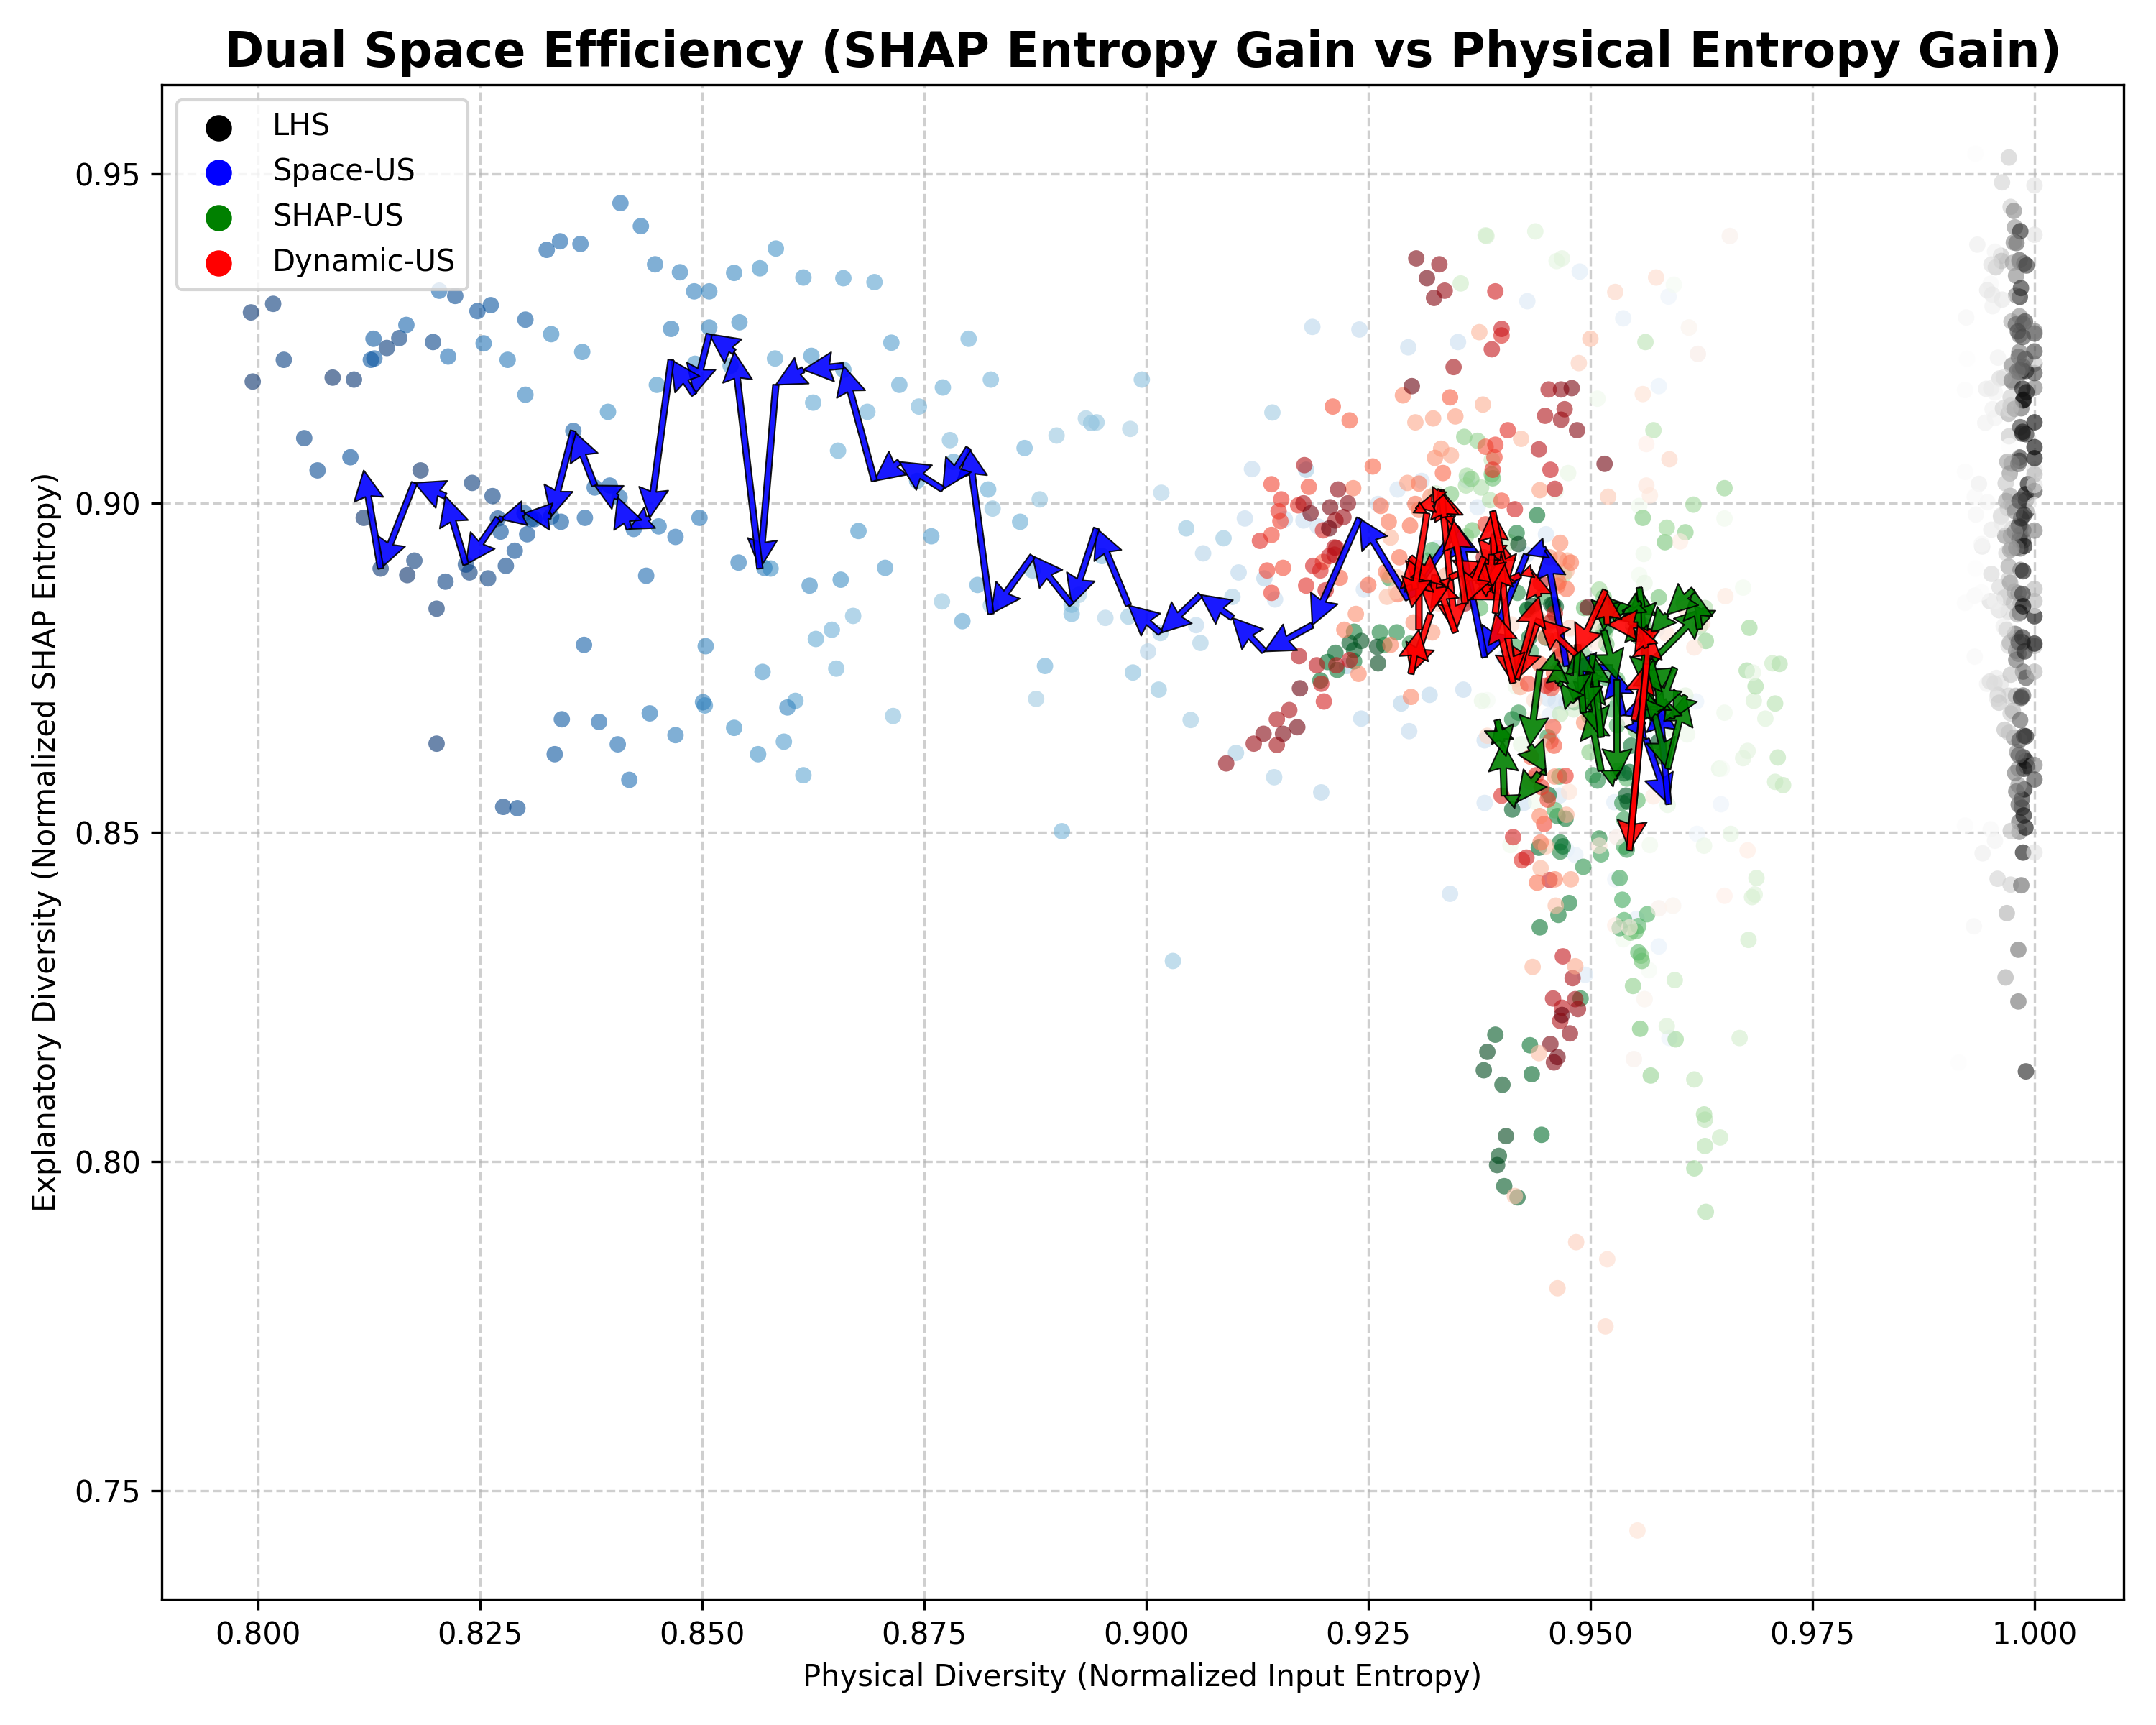
\includegraphics[width=\textwidth]{cireco_final_dual_space_efficiency.png}
      \end{figure}
    \end{column}
  \end{columns}
\end{frame}

\section{Conclusion}

\begin{frame}{Conclusion \& Perspectives}
  \textbf{Contributions:}
  \begin{itemize}
      \item A model-agnostic, multi-fidelity XAI loop that achieves deep structural understanding rather than just raw predictive accuracy.
      \item Demonstrates that optimizing for explanatory diversity uncovers tipping points exponentially faster than classic DoE or SUR.
      \item Validated on robust Agent-Based Models (Cireco, Schelling).
  \end{itemize}
  
  \vspace{0.5cm}
  \textbf{Perspectives:}
  \begin{itemize}
      \item Scaling to more complex ABMs.
      \item Handling highly noisy surrogate environments.
      \item Translating structural understanding into actionable decision-support tools.
  \end{itemize}
\end{frame}

\begin{frame}[standout]
  Questions?
\end{frame}

\end{document}
